% 98-58(98쪽) — $\seg{AB}=8$ · $\seg{BC}=7$ 인 평행사변형 ABCD 와 대각선 $\seg{AC}=13$. 스캔 화질이 낮아 TikZ 로 다시 그림.
% 라벨은 원문 것만: 꼭짓점 A·B·C·D, 길이 8·7·13. 넓이(답)는 적지 않는다.
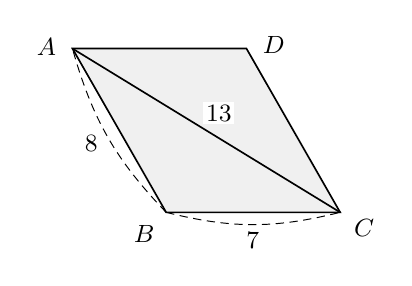
\begin{tikzpicture}[line width=0.6pt, x=1cm, y=1cm]
  \coordinate (A) at (-1.19,2.08);
  \coordinate (B) at (0,0);
  \coordinate (C) at (2.21,0);
  \coordinate (D) at (1.02,2.08);
  \fill[black!6] (A) -- (B) -- (C) -- (D) -- cycle;
  \draw (A) -- (B) -- (C) -- (D) -- cycle;
  \draw (A) -- (C);
  % 길이 표시의 점선 호
  \draw[densely dashed, line width=0.35pt] (B) to[bend left=14] (A);
  \draw[densely dashed, line width=0.35pt] (B) to[bend right=14] (C);
  \node[font=\small, fill=white, inner sep=1pt] at (-0.95,0.87) {$8$};
  \node[font=\small] at (1.10,-0.36) {$7$};
  \node[font=\small, fill=white, inner sep=1pt] at (0.67,1.26) {$13$};
  \node[font=\small, anchor=east] at (-1.27,2.10) {$\pt{A}$};
  \node[font=\small, anchor=north east] at (-0.02,-0.04) {$\pt{B}$};
  \node[font=\small, anchor=north west] at (2.26,0.04) {$\pt{C}$};
  \node[font=\small, anchor=west] at (1.10,2.12) {$\pt{D}$};
\end{tikzpicture}
